\documentclass[11pt,letterpaper,DIV=12]{scrartcl}

\usepackage[T1]{fontenc}
\usepackage[spanish,es-noshorthands]{babel}
\usepackage{lmodern}
\usepackage{graphicx}
\usepackage{booktabs}
\usepackage{tabularx}
\usepackage{longtable}
\usepackage{pdflscape}
\usepackage{array}
\usepackage{xcolor}
\usepackage[hidelinks]{hyperref}
\usepackage{csquotes}
\usepackage[backend=biber,style=apa]{biblatex}

\addbibresource{references.bib}

% Pendientes visibles del equipo
\newcommand{\todo}[1]{{\color{red}\textbf{[TODO: #1]}}}
\newcolumntype{L}[1]{>{\raggedright\arraybackslash}p{#1}}


\setcounter{secnumdepth}{0}

\begin{document}

\titlehead{\centering Instituto Tecnológico y de Estudios Superiores de Monterrey}
\subject{Inteligencia artificial avanzada para la ciencia de datos}
\title{Reporte de entendimiento de los datos}
\subtitle{Grupo 601. Profesores Benjamín Valdés Aguirre y Eduardo Daniel Juárez Pineda}
\author{
  \begin{tabular}{l@{\hspace{2em}}l}
    Facundo Bautista Barbera & Emiliano Camacho Ponce \\
    A01066843 & A01712408 \\[1ex]
    Oswaldo Isaias Hernández Santes & Iker Mejía Hernández \\
    A01199004 & A01352358 \\[1ex]
    Alfredo Alejandro Soto Herrera & Jorge Manuel Oyoqui Aguilera \\
    A01711368 & A01711783
  \end{tabular}
}
\date{\today}

\maketitle


\tableofcontents

\section{Resumen}

El objetivo de minería de datos del proyecto es predecir la condición corporal (BCS) de las vacas del CAETEC. El desempeño del modelo lo vamos a medir con el error absoluto medio (MAE), que nos dice en promedio por cuántos puntos de la escala nos equivocamos, y con la exactitud (Accuracy), que nos dice qué porcentaje de vacas quedan en la clase de BCS correcta. Por eso este reporte empieza con los datos que tienen BCS: las fotografías tomadas en la visita al CAETEC, el BCS asignado por expertos y el dataset de condición corporal de VMS~3. Los datos de ordeño de los robots VMS los describimos después, como contexto y apoyo.

\paragraph{Datos importantes de BCS}
\begin{itemize}
  \item Tenemos 27 valores de BCS asignados por 2 expertos para 24 vacas distintas, de 2.0 a 3.75 en pasos de 0.25, con promedio de 2.95 y mediana de 3.0.
  \item Hay 26 vacas con fotografías clasificadas y un dataset de 24 vacas de VMS~3. Solo 19 vacas tienen dataset y fotos al mismo tiempo.
  \item La columna ``Evento BCS'' del dataset no coincide con el BCS de los expertos, por lo que no la usamos como etiqueta hasta saber qué mide.
  \item Los datos de ordeño solo se cruzan con 3 vacas de BCS (1572, 2082 y 8709).
\end{itemize}

\paragraph{Datos importantes de ordeño}
Describimos los datos de ordeño de 34 vacas registradas por robots de ordeño voluntario (VMS) entre el 01/03/2025 y el 18/07/2025 (140 días). Hay 7,249 registros, de los cuales 7,016 son ordeños, 172 son visitas rechazadas por la máquina y 61 son vacas que no fueron ordeñadas.
\begin{itemize}
  \item Producción: en promedio se generaron 13.7~kg de leche por ordeño y 31.1~kg por día con datos. La producción promedio por ordeño de cada vaca estuvo entre 7.7~kg y 18.9~kg.
  \item Frecuencia: el promedio de ordeños por día es de 2.27. Las vacas tienen un intervalo mediano entre ordeños de entre 7.0 y 14.8 horas.
  \item La cobertura de datos es desigual: tan solo 14 vacas tienen datos en prácticamente todo el rango de 140 días, 12 empiezan después del 01/03/2025 y 6 tienen ausencias prolongadas de entre 54 y 104 días.
  \item Los incidentes se concentran en muy pocas vacas: en promedio ponderado, el 18.5\% de los ordeños presentaron patadas, el 14.5\% están incompletos y el 17.7\% tienen pezones no encontrados. Las medianas por vaca son mucho menores (15.2\%, 8.5\% y 5.1\%), porque unas cuantas vacas, como la 8755, la 8732 o la 6003, concentran los valores más extremos.
  \item Destino de la leche: el 96.5\% de la leche fue al tanque. Hubo \todo{224 o 244, verificar} ordeños cuya leche fue desviada, de los cuales 152 fueron al drenaje y 92 a Divert~3.
  \item Calidad de los datos: las columnas RCS y Usuario están vacías en las 34 vacas y Razón de la desviación tiene un solo valor en todo el conjunto. Dos vacas no tuvieron ninguna lectura en uno de sus cuartos y 25 registros comparten vaca y hora de inicio con otro registro.
\end{itemize}

\noindent\textbf{Nota de verificación.} En la versión de Drive el resumen decía 224 ordeños desviados, pero 152 + 92 = 244, y la sección de destino de la leche también dice 244. Además, $6{,}772 + 152 + 92 = 7{,}016$. Falta confirmar el total con el notebook antes de cerrar este dato.

\section{Adaptaciones a CRISP-DM}

En esta fase hicimos los siguientes ajustes a CRISP-DM:
\begin{itemize}
  \item Juntamos los cuatro entregables de la fase 2 (reporte de recolección inicial, descripción, exploración y calidad) en este documento, en secciones separadas. En Drive están como cuatro reportes (2.1.1, 2.2, 2.3.1 y 2.4.1); esta versión parte del reporte 2.2 y \todo{integrar el contenido de los reportes 2.1.1, 2.3.1 y 2.4.1 de Drive}.
  \item Ordenamos el reporte alrededor del BCS, que es el único objetivo del proyecto. Los datos de ordeño se quedan como contexto porque casi no se cruzan con las vacas que tienen BCS.
  \item Hicimos el análisis en un notebook de Python (pandas) en Google Colab, guardado en \texttt{src/notebooks/01\_reporte\_de\_datos.ipynb}. \todo{definir si el procesamiento se pasa a PySpark/AWS como pide el contexto del curso}.
  \item Los riesgos que encontramos en los datos los evaluamos con probabilidad, impacto y magnitud, igual que en el plan de riesgos de la fase 1.
\end{itemize}

\section{2.1 Reporte de recolección inicial}

\subsection{Datos de BCS}

Estos datos incluyen fotografías tomadas por nuestros compañeros durante la visita al CAETEC el día 29/09/2026 (con dispositivos \todo{dispositivos usados}) y compartidas a través de una carpeta de Drive. También se nos proporcionó el BCS de las vacas fotografiadas, asignado por 2 expertos ese mismo día, y un nuevo dataset con la información de 24 vacas del grupo VMS~3 (\texttt{VACAS\_VMS\_3\_CONDICION\_CORPORAL}). Las fotos son para que el modelo aprenda la forma de las vacas y así pueda predecir su BCS a partir de su figura, mientras que el dataset aporta información de producción, días desde el parto, estado reproductivo, etc.

\subsection{Datos de ordeño}

Los archivos vinieron de la carpeta compartida con el equipo llamada ``Vacas en establo Marzo - Junio 2025''. A pesar de que el nombre dice que van hasta junio, hay fechas que llegan al 18/07/2025. Se analizaron 34 vacas del CAETEC: 1204, 1221, 1233, 1497, 1554, 1572, 1613, 1624, 1634, 2072, 2076, 2078, 2082, 6003, 6036, 6178, 6191, 6194, 6211, 6232, 6238, 8709, 8712, 8729, 8732, 8755, 8758, 8771, 8775, 8777, 8779, 8782, 8792 y 8794. Cada archivo CSV pertenece a una vaca y todos tienen la misma estructura de 35 columnas.

\subsection{Cómo obtuvimos las cifras}

Todas las cifras de ordeño se calcularon en el notebook \texttt{src/notebooks/01\_reporte\_de\_datos.ipynb}, que lee los CSV desde Google Drive montado en Colab (\texttt{/content/drive/MyDrive/...}). \todo{hacer que el notebook lea los datos desde una ruta configurable fuera del repo para que se pueda reproducir sin Colab}. Los datos no se suben al repositorio. \todo{agregar el notebook o el código que genera las cifras de BCS de las secciones 2.2 a 2.4}.

\begin{itemize}
  \item Ordeños: contamos todas las filas cuyo valor en la columna Acción fuera igual a ``Ordeño''.
  \item Días con datos: contamos las fechas distintas que tuvieran al menos un ordeño. La cobertura propia es los días con datos entre los días del periodo de esa vaca, y la cobertura de ventana es los días con datos entre 140.
  \item Ordeños por día: usamos el valor más alto del número de ordeño de cada día (ya que puede haber ordeño 1, 2 y 3 en un mismo día) entre los días con datos. Los días sin registros no se contaron como cero, sino que no se tomaron en cuenta.
  \item Intervalo: como los CSV no traen esta columna, lo calculamos con la diferencia entre horas de inicio consecutivas de una vaca. Reportamos la mediana por vaca. Hablamos de un hueco cuando hay un intervalo de más de 48 horas.
  \item Producción diaria: la producción total entre los días con datos.
  \item Porcentaje de incidentes: el número de ordeños con el campo de ese incidente no vacío entre los ordeños de esa vaca.
  \item Cifras globales ponderadas: cada vaca pesa según su número de ordeños. Las comparaciones entre vacas usan las 31 vacas que tuvieron al menos 30 ordeños.
  \item Cuartos: son promedios ponderados por ordeños, de modo que los ordeños con más de 6.0~mS/cm o con sangre mayor a 0 se cuentan sobre ordeños, no sobre filas.
\end{itemize}

\section{2.2 Descripción de los datos}

\subsection{BCS asignado por expertos}

Los 2 expertos asignaron el BCS a las vacas el mismo día que se fotografiaron (29/09/2026). Tenemos 27 valores para 24 vacas distintas, que van de 2.0 a 3.75 (promedio de 2.95 y mediana de 3.0), en pasos de 0.25. \todo{fuente de la escala de BCS}. A algunas vacas se les dio la etiqueta ``fresca'', que significa recién parida; es decir, está empezando su curva de lactancia, por lo que se espera que su BCS baje. Hubo 3 vacas que aparecieron dos veces en la lista: la 1569 con 2.75 y 2.5 de BCS, la 1561 con 3.25 y 3.0, y la 1644 con 2.5 en ambas.

\subsection{Fotografías}

\begin{itemize}
  \item Hay una carpeta por ID de vaca que contiene imágenes .HEIC, .jpeg y .jpg, y el número de fotos por vaca varía.
  \item De momento hay 26 vacas con fotografías clasificadas, mientras que el resto de las vacas que se fotografiaron sigue sin clasificarse.
  \item \todo{número total de fotos, número de fotos por vaca y número de vacas sin clasificar}.
\end{itemize}

\subsection{Dataset de condición corporal (VMS 3)}

El archivo tiene 24 vacas (una fila por vaca) y 16 columnas. Todas son atendidas por VMS~3. En estado reproductivo hay 11 preñadas, 7 frescas y 6 inseminadas.

\begin{small}
\begin{longtable}{L{4cm}L{4.5cm}L{6.5cm}}
\caption{Columnas del dataset de condición corporal.}\\
\toprule
Columna & Qué representa & Observación en los datos \\
\midrule
\endfirsthead
\toprule
Columna & Qué representa & Observación en los datos \\
\midrule
\endhead
\bottomrule
\endfoot
Número del animal & ID de la vaca. & Hay 24 IDs distintos, algunos de cinco dígitos (como 91549, 91561, 91576, 91578). \\
Nombre del grupo & Grupo de manejo. & Todas son ``VMS 3''. \\
Número(s) de selección de animal & Número de selección. & Es 6 en todas. Falta confirmar qué significa. \\
Estado de la reproducción & Estado reproductivo actual de la vaca. & Preñada (11), Fresca (7), Inseminada (6). \\
Días en ordeño & Días desde que inició su lactancia actual. & De 2 a 391, con mediana de 209.5. \\
Nº Lactación & Número de lactancia. & De 1 a 5, con mediana de 2. \\
Días preñada & Días de gestación. & Solo en las 11 vacas preñadas. Va de 80 a 203 días. \\
Fecha de parto esperada & Fecha esperada del siguiente parto. & Solo en las 11 vacas preñadas. Va del 25/12/2026 al 27/04/2027. \\
Producción media diaria últimos 7 días & Producción diaria promedio reciente (kg). & De 14.89 a 46.44, con mediana de 26.13. \\
Producción TOTAL en lactación & Leche acumulada en la lactancia (kg). & De 23.61 a 17,080.62. \\
Fecha de nacimiento & Fecha de nacimiento de la vaca. & Del 06/06/2019 al 31/07/2024. \\
Fecha de último BCS & Fecha de la última medición de BCS. & Vacía en 9 de 24 vacas; las fechas van del 04/09/2025 al 02/10/2026. \\
Producción ayer en la sesión 1 & Producción de la sesión 1 del día anterior (kg). & De 4.44 a 23.61. No sabemos a qué día se refiere ``ayer''. \\
BCS ayer & BCS del día anterior. & Vacía en las 24 vacas. \\
Tendencia BCS últimas 2 sem. & Cambio del BCS en las últimas 2 semanas. & Solo tiene valor en 7 vacas y va de $-0.5$ a 0.5. \\
Evento BCS & Sus valores parecen ser BCS. & Tiene valor en 19 vacas, de 2.98 a 4.17. Falta confirmar qué mide. \\
\end{longtable}
\end{small}

\subsection{Datos de ordeño}

\paragraph{Qué es cada fila.} Cada fila representa un evento en el robot VMS, no necesariamente un ordeño. La columna Acción tiene tres tipos:
\begin{itemize}
  \item Ordeño (7,016 filas, 96.8\%): la vaca fue ordeñada y se registraron datos de producción, flujos, sangre, conductividad, etc.
  \item Rechazada (172 filas): la vaca se formó, pero el robot no la dejó entrar al ordeño, probablemente porque ya se había formado muchas veces ese día o porque su intervalo entre ordeños fue muy corto.
  \item Echada sin ordeñar (61 filas): ocurre, por ejemplo, al inicio de la lactancia, cuando la vaca no asiste a ordeñarse.
\end{itemize}
Las 233 filas que no son ordeños coinciden exactamente con las 233 filas donde no hay Destino de la leche ni Estado AMD de ubre, lo que confirma que no son ordeños. Por eso las excluimos de todas las estadísticas de producción.

\paragraph{Cuartos de la ubre.} Varias columnas se repiten una vez por cuarto: DD (delantero derecho), DI (delantero izquierdo), TD (trasero derecho) y TI (trasero izquierdo).

\paragraph{Formato del archivo.} Cada CSV viene con un encabezado de dos niveles: el primero indica el grupo (por ejemplo, ``Sangre (ppm)'') y el segundo el cuarto. Al leerlos combinamos los dos niveles en un solo nombre, por ejemplo ``Sangre (ppm) | DI''. Además:
\begin{itemize}
  \item Las fechas vienen como texto en español, por ejemplo ``01/03/2025 05:37 a.\,m.'', y hay que convertirlas a fecha y hora. Las 7,249 fechas se leyeron sin ningún error.
  \item La duración viene como texto en formato ``mm:ss'' y se convierte a segundos.
  \item Las columnas Patada, Incompleto, Pezones no encontrados y AMD Pezón no son ceros y unos: contienen el cuarto afectado (por ejemplo, DI) o varios separados por coma (``DI, TD''), y quedan vacías si no se presentó el evento.
  \item Los 34 archivos tienen exactamente el mismo esquema de columnas.
  \item Estos CSV no incluyen varias columnas que sí aparecían en el dataset de la vaca 6229, como Intervalo de ordeño, Contadores de monitorización, Programa de lavado, MS y MDI. El intervalo entre ordeños ahora lo calculamos nosotros a partir de la hora de inicio; la columna EO/PO toma los mismos valores (VMS 1, 2 y 3) que MS en el dataset de ejemplo.
\end{itemize}

\begin{small}
\begin{longtable}{L{3.6cm}L{5.4cm}L{6cm}}
\caption{Columnas de los datos de ordeño.}\\
\toprule
Columna & Qué representa & Observación en los datos \\
\midrule
\endfirsthead
\toprule
Columna & Qué representa & Observación en los datos \\
\midrule
\endhead
\bottomrule
\endfoot
Hora de inicio & Fecha y hora en la que empezó el evento. & Sin datos vacíos. Va del 01/03/2025 al 18/07/2025. \\
Acción & Tipo de evento: Ordeño, Rechazada o Echada sin ordeñar. & 7,016, 172 y 61 filas respectivamente. \\
Duración (mm:ss) & Tiempo que duró el evento. & El promedio por vaca fue de 5.4 a 13.5 minutos. \\
Producción (kg) & Leche total del ordeño. & Hubo ordeños con 0~kg en 4 vacas (1554, 2078, 6232 y 8782) y con 0.08~kg en la 8712. \\
Estado | Número de ordeño & Número de ordeño de la vaca en ese día. & Sin datos vacíos. \\
Estado | RCS (x1000 células/ml) & Recuento de células somáticas. & Vacía en las 34 vacas. \\
Estado | Patada, Incompleto, Pezones no encontrados & Incidentes del ordeño y el cuarto afectado. ``Incompleto'' es cualquier razón por la que la máquina lo marcó así, aunque no indica cuál fue. & Cuando está vacío significa que no se registró el incidente. \\
Estado AMD | Ubre & Estado de la detección automática de mastitis (AMD) para la ubre. Toma los valores 0 y 1. & El 1 aparece en el 15.0\% de los ordeños. Falta confirmar su significado. \\
Estado AMD | Pezón & Cuartos con aviso de AMD. & Vacía en el 88.9\% de las filas. Falta confirmar su significado. \\
Media de los flujos (kg/min) por cuarto & Velocidad promedio de salida de la leche en cada cuarto. & Un valor por cuarto. \\
Flujos máximos (kg/min) por cuarto & Velocidad máxima de salida de la leche en cada cuarto. & Un valor por cuarto. \\
Producciones (kg) por cuarto & Leche producida por cada cuarto en el ordeño. & Hay dos vacas con un cuarto sin ninguna lectura. \\
Sangre (ppm) por cuarto & Sangre detectada en la leche de cada cuarto. & Normalmente vale 0. \\
Conductividad (mS/cm) por cuarto & Conductividad eléctrica de la leche. El rango común es de 3.0 a 5.0~mS/cm; los valores altos pueden indicar inflamación o mastitis. \todo{fuente del rango y del umbral} & Usamos 6.0~mS/cm como valor alto. \\
Misc | EO/PO & Unidad de ordeño robótica (VMS) que atendió a la vaca. & Solo aparecen las tres máquinas del CAETEC: VMS 1, VMS 2 y VMS 3. \\
Misc | Usuario & El operador. & Vacía en las 34 vacas. El socio confirmó que no hay datos de personas y que la columna no se usa. \\
Misc | Destino Leche & A dónde fue la leche: Tanque, Drenaje o Divert~3. & Vacía solo en las 233 filas que no son ordeños. \\
Misc | Razón de la desviación & Motivo por el que se desvió la leche. & Tiene un único valor (``Separada manualmente'') y está vacía en casi todos los registros, así que no explica los ordeños desviados. \\
\end{longtable}
\end{small}

\section{2.3 Exploración de los datos}

\subsection{Distribución del BCS y su relación con MAE y Accuracy}

\todo{figura e histograma de la distribución del BCS por clase (2.0 a 3.75), con el número de vacas en cada clase}. Esta distribución es importante para las dos métricas: con pocas vacas por clase, la Accuracy puede cambiar mucho con un solo error, y el MAE depende de qué tan lejos quedan las clases extremas (2.0 y 3.75) del centro de la distribución.

\subsection{Cruce entre fotos, dataset y BCS de expertos}

En total tenemos 31 vacas distintas entre las fotografiadas y las del dataset. La tabla siguiente muestra qué información tiene cada una. La columna ``Evento BCS'' es la del dataset; como desconocemos qué significa, no se debe comparar directamente con el BCS de los expertos hasta saber qué mide.

\begin{small}
\begin{longtable}{lccll}
\caption{Información disponible por vaca.}\label{tab:cruce}\\
\toprule
Vaca & En el dataset & Fotos clasificadas & BCS de expertos (29/09/2026) & Evento BCS \\
\midrule
\endfirsthead
\toprule
Vaca & En el dataset & Fotos clasificadas & BCS de expertos (29/09/2026) & Evento BCS \\
\midrule
\endhead
\bottomrule
\endfoot
1213 & Sí & Sí & 2.0 & 4.00 \\
1532 & Sí & Sí & 3.5 & 3.25 \\
1538 & Sí & Sí & 3.0 & 3.00 \\
1543 & Sí & Sí & 3.5 & — \\
1547 & Sí & Sí & 2.75 & 3.98 \\
1549 & No & Sí & — & — \\
1561 & No & Sí & 3.25 y 3.0 & — \\
1564 & Sí & Sí & 3.0 & 3.74 \\
1565 & Sí & Sí & 3.0 (fresca) & — \\
1567 & Sí & Sí & 3.0 & 3.50 \\
1569 & No & Sí & 2.75 y 2.5 (fresca) & — \\
1570 & Sí & No & — & 3.81 \\
1572 & No & Sí & — & — \\
1578 & No & Sí & 3.0 & — \\
1644 & Sí & Sí & 2.5 (aparece dos veces) & 3.93 \\
2082 & Sí & Sí & 3.25 & 3.00 \\
2126 & Sí & Sí & 3.5 & — \\
2142 & Sí & Sí & 3.5 & 3.50 \\
2165 & Sí & No & — & 3.25 \\
6137 & Sí & Sí & 3.75 & 3.79 \\
6226 & Sí & Sí & 2.75 & 3.15 \\
8709 & Sí & Sí & 2.75 & 3.22 \\
8736 & No & Sí & 3.25 (fresca) & — \\
8744 & Sí & Sí & 3.25 (fresca) & 4.17 \\
8769 & Sí & No & — & 2.98 \\
8799 & Sí & Sí & 2.75 & 3.50 \\
91549 & Sí & Sí & 3.0 & 3.48 \\
91561 & Sí & No & — & 3.00 \\
91576 & Sí & Sí & 2.25 (fresca) & — \\
91578 & Sí & No & — & — \\
91579 & No & Sí & 2.5 & — \\
\end{longtable}
\end{small}

En general:
\begin{itemize}
  \item 19 vacas están en el dataset y tienen fotos clasificadas.
  \item 5 vacas están en el dataset pero no tienen fotos clasificadas: 1570, 2165, 8769, 91561 y 91578.
  \item 7 vacas tienen fotos pero no están en el dataset: 1549, 1561, 1569, 1572, 1578, 8736 y 91579.
  \item 2 vacas (1549 y 1572) tienen fotos clasificadas pero no BCS asignado por los expertos.
\end{itemize}

\subsection{Relación con los datos de ordeño}

Los datos de ordeño (34 vacas) casi no corresponden a las vacas con BCS. Solo 3 vacas aparecen en ambos conjuntos: 1572, 2082 y 8709. De ellas, la 2082 y la 8709 están en el dataset, tienen fotos y BCS de expertos (3.25 y 2.75 respectivamente), así que son las únicas con ordeño, fotos, dataset y BCS completos. La 1572 tiene ordeño y fotos, pero no está en el dataset ni tiene BCS de expertos. Por eso los datos de ordeño sirven como contexto, y para entrenar con BCS vamos a depender sobre todo de las fotos y del nuevo dataset.

\subsection{Exploración de los datos de ordeño}

La siguiente tabla resume las principales variables. La columna ``Global'' pondera a cada vaca por su número de ordeños. Las otras columnas comparan a las vacas entre sí y usan solo las 31 vacas con al menos 30 ordeños, ya que tres vacas (1497, 8771 y 8775) tienen muy pocos datos para que sus promedios sean comparables.

\begin{small}
\begin{longtable}{L{4cm}rrrrr}
\caption{Resumen global de los datos de ordeño.}\\
\toprule
Variable & Global & Media entre vacas & Mediana entre vacas & Mínimo & Máximo \\
\midrule
\endfirsthead
\bottomrule
\endfoot
Ordeños por vaca & 7,016 en total (34 vacas) & 206.4 & 244.5 & 1 & 419 \\
Producción por ordeño (kg) & 13.72 & 13.53 & 13.86 & 7.66 & 18.85 \\
Producción diaria (kg) & 31.12 & 30.45 & 28.13 & 13.15 & 55.50 \\
Ordeños por día & 2.27 & 2.21 & 2.14 & 1.45 & 3.17 \\
Duración media (min) & 8.48 & 8.24 & 7.83 & 5.36 & 13.51 \\
Ordeños con patada (\%) & 18.5 & 18.2 & 15.2 & 0.7 & 62.2 \\
Ordeños incompletos (\%) & 14.5 & 13.8 & 8.5 & 0.0 & 57.9 \\
Ordeños con pezones no encontrados (\%) & 17.7 & 16.3 & 5.1 & 0.0 & 83.3 \\
\end{longtable}
\end{small}

\noindent La producción diaria es la producción total entre los días en que la vaca tuvo al menos un ordeño. El global incluye a las 34 vacas.

\begin{figure}[htbp]
  \centering
  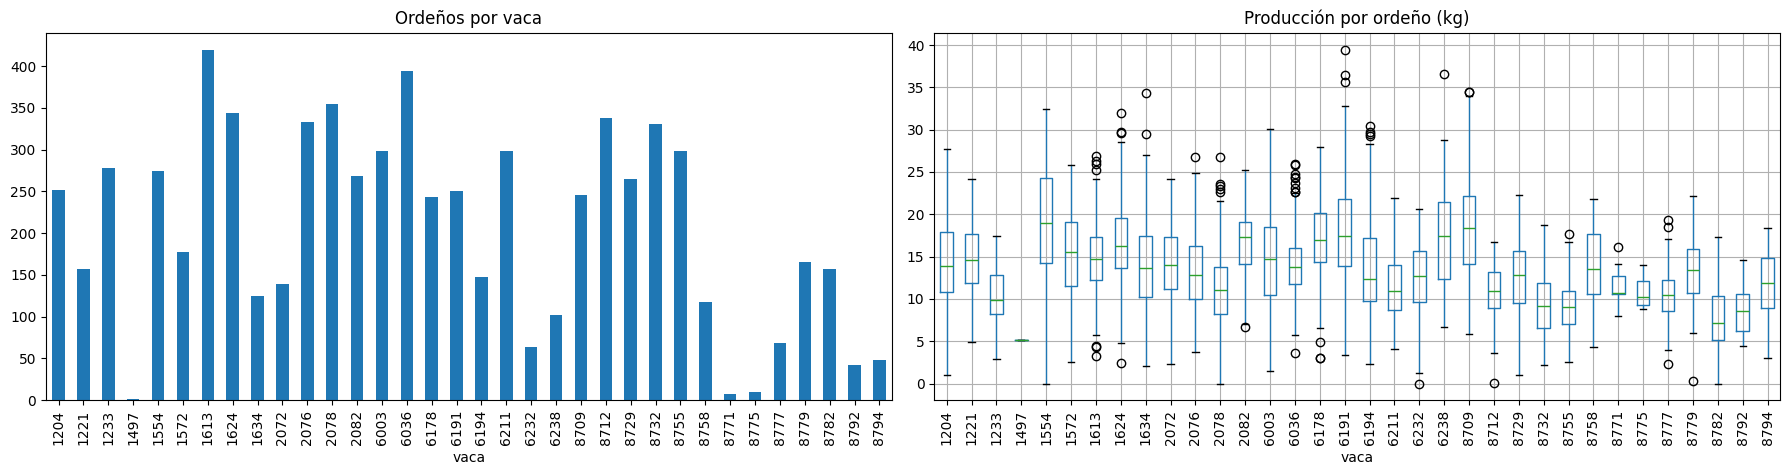
\includegraphics[width=\textwidth]{figures/ordenos_produccion_por_vaca.png}
  \caption{Ordeños por vaca y producción por ordeño (kg) por vaca. Generada en la celda 4 del notebook \texttt{01\_reporte\_de\_datos.ipynb}.}
  \label{fig:ordenos}
\end{figure}

\paragraph{Producción, frecuencia y duración.}
\begin{itemize}
  \item Producción: el promedio global fue de 13.7~kg por ordeño y la mediana entre vacas de 13.9~kg. La vaca con mayor promedio fue la 1554 con 18.9~kg por ordeño, y la de menor promedio entre las comparables fue la 8782 con 7.7~kg. El ordeño más grande fue de la vaca 6191, con 39.5~kg (figura~\ref{fig:ordenos}).
  \item Ordeños con producción casi nula: cinco vacas tuvieron ordeños con 0~kg o 0.08~kg: 1554, 2078, 6232, 8782 y 8712. El socio formador recomendó hacer una auditoría para entender qué pasó con estas vacas antes de empezar a modelar.
  \item Frecuencia: las vacas se ordeñan en promedio 2.27 veces al día. El mínimo entre las comparables fue de 1.45 y el máximo de 3.17 (vaca 6003). El intervalo mediano entre ordeños va de 7.0~h (6003) a 14.8~h (8792 y 8794), con un promedio cercano a 10.5~h.
  \item Duración: un ordeño dura en promedio 8.5 minutos. La vaca más rápida promedió 5.4 minutos (8712) y la más lenta 13.5 minutos (8755). \todo{en la versión de Drive decía 8782, pero en la tabla A2 la duración media de 13.5 min es de la 8755; confirmar}
\end{itemize}

\paragraph{Comportamiento por cuarto.} La tabla tiene los promedios ponderados por ordeños. Las dos vacas con un cuarto sin datos (6211 y 6232) quedaron fuera del cálculo de ese cuarto.

\begin{small}
\begin{longtable}{lrrrrrr}
\caption{Valores por cuarto.}\\
\toprule
Cuarto & Prod. media (kg) & Flujo mediano (kg/min) & Flujo máximo (kg/min) & Conductividad media (mS/cm) & Ordeños > 6.0 mS/cm & Ordeños con sangre > 0 \\
\midrule
\endfirsthead
\bottomrule
\endfoot
TD & 3.88 & 1.07 & 1.54 & 3.82 & 1.98\% & 63 \\
TI & 3.59 & 1.05 & 1.49 & 4.38 & 0.88\% & 150 \\
DD & 3.26 & 1.11 & 1.58 & 4.74 & 0.93\% & 100 \\
DI & 3.18 & 1.03 & 1.50 & 4.65 & 2.81\% & 118 \\
\end{longtable}
\end{small}

\begin{itemize}
  \item Producción: los cuartos traseros producen más que los delanteros. TD produce 3.88~kg y TI 3.59~kg, mientras que DD produce 3.26~kg y DI 3.18~kg.
  \item Hay fuertes asimetrías: en varias vacas hay cuartos que producen mucho más que los demás. En la 1233, el cuarto TI promedia 0.82~kg y el TD 3.44~kg. En la 8755, el TD promedia 1.16~kg frente a 4.13~kg del DD. En la 2082, el DD promedia 1.75~kg y el TI 5.29~kg.
  \item Cuartos sin datos: en la vaca 6211 en el cuarto TI y en la 6232 en el cuarto TD no hay valores de producción, flujos, sangre ni conductividad. Según el socio formador, ese cuarto no se está ordeñando. Puede tratarse de una situación anterior donde haya cicatrizado el tejido, por lo que es un problema de salud y es posible que haya vacas con un cuarto sin datos en toda la serie.
  \item Flujos: los flujos entre cuartos se parecen. La media va de 1.03 a 1.11~kg/min y el máximo de 1.49 a 1.58~kg/min.
  \item Conductividad: la media va de 3.82~mS/cm (TD) a 4.74~mS/cm (DD). Los ordeños con más de 6.0~mS/cm son pocos en todos los cuartos (entre 0.9\% y 2.8\%), pero se concentran en algunas vacas: la 6178 en el DI con 23.1\%, la 6191 en el DI con 19.6\%, la 8755 en el TD con 15.7\% y la 6238 en el TD con 15.7\%.
  \item Sangre: únicamente 431 lecturas de cuarto tienen sangre mayor a 0~ppm, menos del 2\% del total. La vaca 2078 tiene 52 de estas lecturas en el cuarto TI, que es la mayor concentración, seguida de la 8782 con 22 lecturas en TI y la 1572 con 19 en DI.
\end{itemize}

\paragraph{Incidentes de ordeño.} Esta tabla de conteos usa los 7,249 registros y separa los incidentes que afectaron a un solo cuarto de los que afectaron a varios.

\begin{small}
\begin{longtable}{L{5.5cm}rrrr}
\caption{Incidentes por cuarto.}\\
\toprule
Cuarto & Patada & Incompleto & Pezones no encontrados & AMD Pezón \\
\midrule
\endfirsthead
\bottomrule
\endfoot
DI (solo ese cuarto) & 350 & 116 & 220 & 257 \\
DD (solo ese cuarto) & 102 & 54 & 59 & 65 \\
TI (solo ese cuarto) & 175 & 367 & 454 & 143 \\
TD (solo ese cuarto) & 512 & 191 & 264 & 215 \\
Combinaciones más frecuentes de dos cuartos & 101 & 172 & 162 & 72 \\
Combinaciones menos frecuentes & 59 & 114 & 80 & 50 \\
Total de registros con el evento & 1,299 & 1,014 & 1,239 & 802 \\
\end{longtable}
\end{small}

\begin{itemize}
  \item La patada se da sobre todo en el cuarto TD, con 512 casos en solitario, más los que aparecen en combinación con TD.
  \item Los ordeños incompletos y los pezones no encontrados se dan sobre todo en el cuarto TI, con 367 y 454 casos en solitario respectivamente.
  \item Estos incidentes están muy concentrados. Las vacas 8755, 8732 y 6003 tienen entre 45\% y 83\% de sus ordeños con pezones no encontrados o incompletos, y la 2076 tiene patada en el 62.2\% de sus ordeños. Hay 4 vacas (1497, 8771, 8775 y 6232) con 0\% de incompletos, pero 3 de ellas tienen muy pocos datos.
\end{itemize}

\paragraph{Estado AMD.} El estado AMD de la ubre vale 1 en 1,050 de los 7,016 ordeños (15.0\%) y 0 en los demás. El campo AMD de pezón indica el cuarto en 802 registros, sobre todo DI (257), TD (215) y TI (143). Según el socio formador, el significado del 1 debe confirmarse con el CAETEC, así que por ahora solo consideramos su frecuencia.

\paragraph{Destino de la leche.}

\begin{small}
\begin{longtable}{lrr}
\caption{Destino de la leche.}\\
\toprule
Destino & Ordeños & Porcentaje \\
\midrule
\endfirsthead
\bottomrule
\endfoot
Tanque & 6,772 & 96.5\% \\
Drenaje & 152 & 2.2\% \\
Divert 3 & 92 & 1.3\% \\
Total de ordeños & 7,016 & 100\% \\
\end{longtable}
\end{small}

\begin{itemize}
  \item Desviar la leche significa que su destino no es el tanque, donde se mezcla la leche de todas las vacas. Según el socio formador, si la leche tiene sangre o microbios se desecha. El socio no pudo confirmarnos qué es Divert~3, así que lo tenemos que revisar con el CAETEC.
  \item Trece vacas enviaron menos del 95\% de su leche al tanque. El caso más destacable es la 6003, que solo envió el 71.5\% al tanque (213 de 298 ordeños, celda 4 del notebook); le siguen dos vacas con muy pocos ordeños, la 8771 (14.3\% al tanque) y la 8775 (0\%).
  \item La columna Razón de la desviación tiene un único valor en todo el conjunto, así que no explica los \todo{224 o 244, verificar} ordeños desviados. Para entenderlos tendríamos que cruzar el destino con sangre, conductividad y AMD, sin suponer la causa antes de tiempo.
\end{itemize}

\paragraph{Robots de ordeño.} Sobre las 7,249 filas: VMS~3 registró 4,276 (59.0\%), VMS~2 registró 1,674 (23.1\%) y VMS~1 registró 1,299 (17.9\%).

\paragraph{Cobertura temporal.}
\begin{itemize}
  \item Cobertura completa: hay 14 vacas con datos en al menos el 97\% de los 140 días, como la 1613, 1624, 2076, 2078, 2082, 6036 y 6211.
  \item Entrada tardía: 12 vacas empezaron después del 01/03/2025. Por ejemplo, la 1497 solo tiene un ordeño (el 18/07/2025), la 8771 y la 8775 empezaron el 14/07/2025 y la 6003 el 16/04/2025.
  \item Ausencias largas: seis vacas tuvieron datos en menos del 60\% de su propio periodo, con huecos máximos de entre 54 y 104 días: la 6232 con 22.1\% y un hueco de 104 días, la 1634 con 37.9\%, la 6238 con 38.6\%, la 1221 y la 6194 con 45.7\% y la 2072 con 51.4\%. El socio formador explicó que estos huecos pueden corresponder al periodo seco de la vaca, cuando está por iniciar otra lactancia.
\end{itemize}

\section{2.4 Calidad de los datos}

\subsection{Calidad de los datos de BCS}

\begin{itemize}
  \item Cobertura desigual: de 31 vacas, solo 19 tienen a la vez dataset y fotos, así que solo esas se pueden usar completas para entrenar y evaluar con las variables del dataset.
  \item Muestra pequeña: solo hay 24 vacas en el dataset y 26 con fotos clasificadas, y el número de fotos por vaca varía.
  \item ``BCS ayer'' está vacía en las 24 vacas, mientras que ``Evento BCS'' tiene valores parecidos a un BCS. Necesitamos confirmar si se relacionan y qué significan.
  \item ``Evento BCS'' no coincide con el BCS de los expertos. De 15 vacas con ambos valores, el del dataset es mayor en 11, igual en 2 y menor en 2. La mayor diferencia está en la 1213 (2.0 de los expertos contra 4.0 del dataset), seguida de la 1644 (2.5 contra 3.93) y la 1547 (2.75 contra 3.98). No lo usaremos como etiqueta hasta aclarar qué mide y de qué fecha es.
  \item Hay BCS registrados el 01/10/2026 y el 02/10/2026, justo después de la visita del 29/09/2026, así que el dataset es posterior a la visita, pero los campos de ``ayer'' y ``días en ordeño'' son de fechas que aún tenemos que confirmar.
  \item ``Fecha de último BCS'' está vacía en 9 vacas y en otras es de 2025.
  \item La etiqueta ``fresca'' no coincide con el dataset: los expertos marcaron como frescas a la 8744, 1565 y 91576, que en el dataset están como preñada o inseminada, y la 2126, 1644, 8709 y 8799 son ``Fresca'' en el dataset pero no tienen la etiqueta de los expertos. Hay que auditarlo, porque este dato afecta cómo cambia el BCS de las vacas.
  \item ``Días preñada'' y ``Fecha de parto esperada'' están vacías en las 13 vacas no preñadas, lo cual es esperado. ``Tendencia BCS'' está vacía en 17 vacas y ``Fecha de último BCS'' en 9.
  \item Hay IDs duplicados en la lista de expertos (1569, 1561 y 1644) y vacas con IDs de 5 dígitos (91549, 91561, 91576, 91578 y 91579). Probablemente no son errores de captura, pero conviene confirmarlo.
\end{itemize}

\subsection{Riesgos de las decisiones de etiqueta}

Evaluamos los riesgos con la misma lógica del plan de riesgos: probabilidad (1 a 5), impacto (1 a 5) y magnitud = probabilidad $\times$ impacto. Con magnitud de 12 o más mitigamos; con menos, aceptamos y monitoreamos. \todo{validar en equipo los valores de probabilidad e impacto propuestos}

\begin{small}
\begin{longtable}{L{4.2cm}ccc L{6.3cm}}
\caption{Riesgos de las decisiones de etiqueta pendientes.}\\
\toprule
Riesgo & P & I & M & Decisión \\
\midrule
\endfirsthead
\toprule
Riesgo & P & I & M & Decisión \\
\midrule
\endhead
\bottomrule
\endfoot
BCS distinto para la misma vaca (1561: 3.25 y 3.0; 1569: 2.75 y 2.5) & 5 & 3 & 15 & Mitigar: decidir entre uno de los dos valores o el promedio y documentarlo antes de entrenar. \\
Usar ``Evento BCS'' como etiqueta sin saber qué mide & 3 & 5 & 15 & Mitigar: usar solo el BCS de expertos hasta que el socio confirme qué mide la columna. \\
Etiqueta ``fresca'' contradictoria entre expertos y dataset & 4 & 3 & 12 & Mitigar: auditar las 7 vacas en conflicto con el CAETEC. \\
Pocas vacas por clase de BCS, lo que vuelve inestables la Accuracy y el MAE & 5 & 4 & 20 & Mitigar: completar la clasificación de fotos y separar entrenamiento y prueba por vaca. \\
Fotos sin clasificar que no entren a tiempo & 3 & 3 & 9 & Aceptar y monitorear: agregarlas cuando estén clasificadas. \\
\end{longtable}
\end{small}

\subsection{Calidad de los datos de ordeño}

\begin{small}
\begin{longtable}{L{3.2cm}L{5.6cm}L{6.2cm}}
\caption{Calidad de los datos de ordeño.}\\
\toprule
Aspecto & Evidencia & Tratamiento \\
\midrule
\endfirsthead
\toprule
Aspecto & Evidencia & Tratamiento \\
\midrule
\endhead
\bottomrule
\endfoot
Filas que no son de ordeño & 233 filas con otra acción: 172 rechazadas y 61 echadas sin ordeñar. & Se excluyen de las estadísticas de producción, incidentes y destino. \\
Posibles duplicados & 25 registros comparten vaca y hora de inicio con otro registro (49 filas involucradas; 4 son copias exactas, celda 4 del notebook). La mayoría son un ordeño y una ``Echada sin ordeñar'' a la misma hora. & De momento no se eliminan, por lo que los conteos pueden estar inflados hasta en 25 filas. \\
Columnas vacías & RCS y Usuario están vacías en las 34 vacas y Razón de la desviación en 33. & No aportan información. No interpretamos el vacío de RCS como ausencia de mastitis, sino como que no se registró. El socio confirmó que Usuario no se usa. \\
Cuartos sin lectura & La 6211 (TI) y la 6232 (TD) tienen 5 columnas vacías por cuarto. & Según el socio, son cuartos que no se ordeñan (problema de salud). Se mantienen como faltantes y no se imputan. \\
Vacas con pocos datos & La 1497 tuvo un ordeño, la 8771 tuvo 7 y la 8775 tuvo 10. & Se excluyen de las comparaciones entre vacas y se marcan con asterisco en el anexo A. \\
Huecos largos & Seis vacas con menos del 60\% de cobertura propia y huecos de 54 a 104 días. & Según el socio, corresponden al periodo seco. Sus promedios diarios pueden servir, pero no son comparables entre vacas. \\
Producción en cero & Ordeños con 0~kg en 1554, 2078, 6232 y 8782, y con 0.08~kg en 8712. & Hay que revisar si son ordeños fallidos antes de modelar; queda pendiente la auditoría. También hay que revisar valores imposibles (como valores muy altos). \\
Vacíos que significan ``no ocurrió'' & Patada, Incompleto, Pezones no encontrados y AMD Pezón están vacías entre el 82\% y 89\% de las filas. & No se tratan como faltantes, sino como ausencia del evento. \\
Umbral de conductividad & El rango común es de 3.0 a 5.0~mS/cm y la alerta se da alrededor de 5.5. \todo{fuente} & Usamos 6.0~mS/cm como valor alto; puede ajustarse cuando el socio defina su umbral. \\
\end{longtable}
\end{small}

Fuera de estos detalles, las 7,249 fechas son legibles, los 34 archivos comparten el mismo esquema y las demás columnas numéricas no tienen vacíos en las filas de ordeño, salvo los dos cuartos mencionados.

\subsection{Pendientes por aclarar}

\begin{itemize}
  \item Qué mide ``Evento BCS'', por qué ``BCS ayer'' está vacía y de qué fecha es el archivo.
  \item Qué valor de BCS usar para las vacas 1569 y 1561.
  \item Clasificar las fotos que faltan.
  \item Qué significa el valor 6 de ``Número(s) de selección de animal''.
  \item Qué significan el 1 en Estado AMD y Divert~3 en los datos de ordeño.
\end{itemize}

\clearpage
\section{Anexo A. Detalles de cada vaca}\label{sec:anexo}

Como aclaración, las vacas con asterisco en el ID son aquellas que tienen menos de 30 ordeños, de modo que sus promedios no son comparables. La cobertura propia es relativa al periodo de cada vaca y la cobertura de ventana al total de 140 días. En la versión de Drive las filas de las vacas 2078 y 2082 aparecían con el ID corrido (como 2082 y 6003); las corregimos con la tabla \texttt{resumen} de la celda 4 del notebook, que coincide en ordeños y fechas.

\begin{landscape}
\footnotesize
\begin{longtable}{l>{\raggedleft\arraybackslash}p{1.45cm}>{\raggedleft\arraybackslash}p{1.45cm}>{\raggedleft\arraybackslash}p{1.45cm}>{\raggedleft\arraybackslash}p{1.45cm}>{\raggedleft\arraybackslash}p{1.45cm}>{\raggedleft\arraybackslash}p{1.45cm}>{\raggedleft\arraybackslash}p{1.45cm}>{\raggedleft\arraybackslash}p{1.45cm}>{\raggedleft\arraybackslash}p{1.45cm}>{\raggedleft\arraybackslash}p{1.45cm}>{\raggedleft\arraybackslash}p{1.45cm}>{\raggedleft\arraybackslash}p{1.45cm}}
\caption{Actividad y producción por vaca.}\label{tab:a1}\\
\toprule
Vaca & Ordeños & Primer ordeño & Último ordeño & Días con datos & Cob. propia (\%) & Cob. ventana (\%) & Hueco máx. (días) & Ordeños por día & Intervalo mediano (h) & Prod. media (kg) & Desv. est. (kg) & Prod. diaria (kg)\\
\midrule
\endfirsthead
\toprule
Vaca & Ordeños & Primer ordeño & Último ordeño & Días con datos & Cob. propia (\%) & Cob. ventana (\%) & Hueco máx. (días) & Ordeños por día & Intervalo mediano (h) & Prod. media (kg) & Desv. est. (kg) & Prod. diaria (kg)\\
\midrule
\endhead
\bottomrule
\endfoot
1204 & 252 & 01/03/2025 & 18/07/2025 & 139 & 99.3 & 99.3 & 1.5 & 1.81 & 12.5 & 14.60 & 5.10 & 26.5 \\
1221 & 157 & 01/03/2025 & 18/07/2025 & 64 & 45.7 & 45.7 & 77.2 & 2.45 & 8.7 & 14.67 & 3.95 & 36.0 \\
1233 & 278 & 01/03/2025 & 18/07/2025 & 138 & 98.6 & 98.6 & 2.7 & 2.01 & 10.7 & 10.42 & 3.05 & 21.0 \\
1497$^{*}$ & 1 & 18/07/2025 & 18/07/2025 & 1 & 100.0 & 0.7 & — & 1.00 & — & 5.20 & — & 5.2 \\
1554 & 275 & 01/03/2025 & 18/07/2025 & 115 & 82.1 & 82.1 & 26.0 & 2.39 & 9.6 & 18.85 & 6.75 & 45.1 \\
1572 & 177 & 01/03/2025 & 18/07/2025 & 86 & 61.4 & 61.4 & 54.3 & 2.06 & 11.5 & 15.37 & 5.02 & 31.6 \\
1613 & 419 & 01/03/2025 & 18/07/2025 & 140 & 100.0 & 100.0 & 0.7 & 2.99 & 7.8 & 14.96 & 3.81 & 44.8 \\
1624 & 344 & 01/03/2025 & 18/07/2025 & 140 & 100.0 & 100.0 & 1.1 & 2.46 & 9.2 & 16.98 & 4.90 & 41.7 \\
1634 & 125 & 01/03/2025 & 18/07/2025 & 53 & 37.9 & 37.9 & 87.7 & 2.36 & 8.9 & 14.09 & 5.52 & 33.2 \\
2072 & 139 & 01/03/2025 & 18/07/2025 & 72 & 51.4 & 51.4 & 54.1 & 1.93 & 12.0 & 14.41 & 4.34 & 27.8 \\
2076 & 333 & 01/03/2025 & 18/07/2025 & 140 & 100.0 & 100.0 & 1.0 & 2.38 & 9.4 & 13.36 & 4.43 & 31.8 \\
2078 & 355 & 01/03/2025 & 18/07/2025 & 140 & 100.0 & 100.0 & 0.9 & 2.54 & 8.8 & 11.09 & 4.62 & 28.1 \\
2082 & 269 & 01/03/2025 & 18/07/2025 & 140 & 100.0 & 100.0 & 1.1 & 1.92 & 11.8 & 16.40 & 3.39 & 31.5 \\
6003 & 298 & 16/04/2025 & 18/07/2025 & 94 & 100.0 & 67.1 & 0.8 & 3.17 & 7.0 & 14.68 & 5.90 & 46.5 \\
6036 & 394 & 01/03/2025 & 18/07/2025 & 140 & 100.0 & 100.0 & 0.8 & 2.81 & 8.2 & 14.12 & 3.44 & 39.7 \\
6178 & 243 & 01/03/2025 & 17/07/2025 & 139 & 100.0 & 99.3 & 1.4 & 1.75 & 13.2 & 16.91 & 4.69 & 29.6 \\
6191 & 250 & 29/04/2025 & 18/07/2025 & 81 & 100.0 & 57.9 & 0.6 & 3.09 & 7.3 & 17.98 & 5.92 & 55.5 \\
6194 & 148 & 01/03/2025 & 18/07/2025 & 64 & 45.7 & 45.7 & 70.4 & 2.31 & 9.4 & 13.74 & 5.68 & 31.8 \\
6211 & 299 & 01/03/2025 & 18/07/2025 & 140 & 100.0 & 100.0 & 0.9 & 2.14 & 10.9 & 11.56 & 3.92 & 24.7 \\
6232 & 64 & 01/03/2025 & 18/07/2025 & 31 & 22.1 & 22.1 & 104.3 & 2.06 & 10.3 & 12.46 & 4.82 & 25.7 \\
6238 & 102 & 01/03/2025 & 18/07/2025 & 54 & 38.6 & 38.6 & 85.2 & 1.89 & 10.0 & 17.00 & 5.85 & 32.1 \\
8709 & 246 & 21/04/2025 & 18/07/2025 & 89 & 100.0 & 63.6 & 0.9 & 2.76 & 8.3 & 18.62 & 5.69 & 51.5 \\
8712 & 338 & 01/03/2025 & 18/07/2025 & 138 & 98.6 & 98.6 & 2.7 & 2.45 & 9.2 & 10.92 & 2.72 & 26.7 \\
8729 & 265 & 01/03/2025 & 18/07/2025 & 136 & 97.1 & 97.1 & 1.4 & 1.95 & 11.6 & 12.73 & 4.17 & 24.8 \\
8732 & 331 & 01/03/2025 & 18/07/2025 & 140 & 100.0 & 100.0 & 1.0 & 2.36 & 9.7 & 9.20 & 3.40 & 21.8 \\
8755 & 299 & 01/03/2025 & 17/07/2025 & 138 & 99.3 & 98.6 & 1.1 & 2.17 & 10.8 & 9.16 & 2.86 & 19.8 \\
8758 & 118 & 19/05/2025 & 18/07/2025 & 61 & 100.0 & 43.6 & 1.5 & 1.93 & 11.2 & 13.86 & 4.27 & 26.8 \\
8771$^{*}$ & 7 & 14/07/2025 & 18/07/2025 & 5 & 100.0 & 3.6 & 0.7 & 1.40 & 13.5 & 11.64 & 2.67 & 16.3 \\
8775$^{*}$ & 10 & 14/07/2025 & 18/07/2025 & 5 & 100.0 & 3.6 & 0.6 & 2.00 & 9.0 & 10.84 & 1.97 & 21.7 \\
8777 & 68 & 06/06/2025 & 18/07/2025 & 38 & 88.4 & 27.1 & 2.3 & 1.79 & 11.3 & 10.17 & 3.41 & 18.2 \\
8779 & 165 & 19/04/2025 & 18/07/2025 & 84 & 92.3 & 60.0 & 3.0 & 1.96 & 10.9 & 13.34 & 3.83 & 26.2 \\
8782 & 157 & 16/04/2025 & 18/07/2025 & 89 & 94.7 & 63.6 & 2.3 & 1.76 & 12.8 & 7.66 & 3.79 & 13.5 \\
8792 & 42 & 21/06/2025 & 18/07/2025 & 27 & 96.4 & 19.3 & 1.5 & 1.56 & 14.8 & 8.45 & 2.51 & 13.2 \\
8794 & 48 & 12/06/2025 & 18/07/2025 & 33 & 89.2 & 23.6 & 1.8 & 1.45 & 14.8 & 11.54 & 3.96 & 16.8 \\
\end{longtable}
\end{landscape}
\begin{landscape}
\footnotesize
\begin{longtable}{l>{\raggedleft\arraybackslash}p{1.45cm}>{\raggedleft\arraybackslash}p{1.45cm}>{\raggedleft\arraybackslash}p{1.45cm}>{\raggedleft\arraybackslash}p{1.45cm}>{\raggedleft\arraybackslash}p{1.45cm}>{\raggedleft\arraybackslash}p{1.45cm}>{\raggedleft\arraybackslash}p{1.45cm}>{\raggedleft\arraybackslash}p{1.45cm}>{\raggedleft\arraybackslash}p{1.45cm}>{\raggedleft\arraybackslash}p{1.45cm}>{\raggedleft\arraybackslash}p{1.45cm}}
\caption{Incidentes, destino de la leche y calidad por vaca.}\label{tab:a2}\\
\toprule
Vaca & Ordeños & Visitas rechazadas & Echada sin ordeñar & Duración media (min) & Patada (\%) & Incompleto (\%) & Pezones no enc. (\%) & Leche a tanque (\%) & Prod. mín. (kg) & Prod. máx. (kg) & Columnas vacías\\
\midrule
\endfirsthead
\toprule
Vaca & Ordeños & Visitas rechazadas & Echada sin ordeñar & Duración media (min) & Patada (\%) & Incompleto (\%) & Pezones no enc. (\%) & Leche a tanque (\%) & Prod. mín. (kg) & Prod. máx. (kg) & Columnas vacías\\
\midrule
\endhead
\bottomrule
\endfoot
1204 & 252 & 7 & 0 & 7.6 & 6.8 & 11.1 & 7.1 & 100.0 & 1.05 & 27.7 & 3 \\
1221 & 157 & 4 & 1 & 7.5 & 14.0 & 3.8 & 3.2 & 92.4 & 4.86 & 24.2 & 3 \\
1233 & 278 & 17 & 1 & 8.7 & 33.1 & 19.4 & 44.2 & 100.0 & 2.89 & 17.4 & 3 \\
1497$^{*}$ & 1 & 0 & 1 & 6.3 & 0.0 & 0.0 & 0.0 & 0.0 & 5.20 & 5.2 & 7 \\
1554 & 275 & 1 & 2 & 7.9 & 11.3 & 14.6 & 12.4 & 100.0 & 0.00 & 32.5 & 3 \\
1572 & 177 & 8 & 1 & 7.0 & 7.9 & 1.7 & 1.7 & 93.8 & 2.49 & 25.8 & 3 \\
1613 & 419 & 1 & 1 & 9.2 & 24.3 & 3.8 & 2.6 & 100.0 & 3.31 & 26.8 & 4 \\
1624 & 344 & 5 & 2 & 7.3 & 8.7 & 3.2 & 3.2 & 100.0 & 2.39 & 32.0 & 3 \\
1634 & 125 & 5 & 2 & 9.6 & 12.0 & 20.0 & 24.8 & 100.0 & 2.05 & 34.4 & 3 \\
2072 & 139 & 2 & 3 & 7.4 & 25.9 & 5.0 & 5.0 & 91.4 & 2.28 & 24.2 & 3 \\
2076 & 333 & 7 & 1 & 7.0 & 62.2 & 9.6 & 6.6 & 100.0 & 3.74 & 26.8 & 3 \\
2078 & 355 & 12 & 5 & 8.7 & 12.4 & 23.4 & 23.4 & 100.0 & 0.00 & 26.8 & 3 \\
2082 & 269 & 20 & 0 & 7.8 & 6.7 & 1.5 & 1.1 & 100.0 & 6.66 & 25.3 & 3 \\
6003 & 298 & 0 & 2 & 9.0 & 7.4 & 45.0 & 50.3 & 71.5 & 1.45 & 30.1 & 3 \\
6036 & 394 & 14 & 2 & 9.3 & 21.3 & 3.0 & 2.8 & 100.0 & 3.66 & 25.9 & 3 \\
6178 & 243 & 4 & 2 & 8.0 & 20.2 & 10.3 & 10.3 & 93.4 & 3.04 & 27.9 & 3 \\
6191 & 250 & 2 & 1 & 10.3 & 18.8 & 15.2 & 13.6 & 100.0 & 3.37 & 39.5 & 3 \\
6194 & 148 & 1 & 1 & 6.6 & 0.7 & 4.0 & 3.4 & 99.3 & 2.33 & 30.5 & 3 \\
6211 & 299 & 14 & 3 & 8.3 & 23.1 & 2.0 & 2.0 & 86.6 & 4.05 & 21.9 & 8 \\
6232 & 64 & 5 & 0 & 6.7 & 6.3 & 0.0 & 1.6 & 85.9 & 0.00 & 20.6 & 10 \\
6238 & 102 & 2 & 1 & 6.8 & 23.5 & 4.9 & 3.9 & 89.2 & 6.66 & 36.5 & 3 \\
8709 & 246 & 0 & 2 & 9.0 & 31.7 & 3.7 & 2.9 & 96.8 & 5.83 & 34.5 & 3 \\
8712 & 338 & 8 & 4 & 5.4 & 3.0 & 4.7 & 3.5 & 100.0 & 0.08 & 16.7 & 3 \\
8729 & 265 & 8 & 0 & 7.6 & 1.1 & 10.2 & 7.2 & 100.0 & 1.05 & 22.3 & 3 \\
8732 & 331 & 8 & 2 & 12.2 & 30.5 & 48.3 & 77.6 & 100.0 & 2.17 & 18.7 & 2 \\
8755 & 299 & 1 & 2 & 13.5 & 21.1 & 57.9 & 83.3 & 100.0 & 2.58 & 17.7 & 3 \\
8758 & 118 & 0 & 7 & 5.6 & 8.5 & 8.5 & 5.1 & 95.8 & 4.32 & 21.8 & 3 \\
8771$^{*}$ & 7 & 0 & 1 & 7.1 & 28.6 & 0.0 & 0.0 & 14.3 & 7.99 & 16.1 & 5 \\
8775$^{*}$ & 10 & 0 & 0 & 6.0 & 10.0 & 0.0 & 0.0 & 0.0 & 8.82 & 14.0 & 5 \\
8777 & 68 & 7 & 0 & 10.0 & 26.5 & 23.5 & 25.0 & 94.1 & 2.26 & 19.3 & 3 \\
8779 & 165 & 5 & 4 & 6.5 & 15.2 & 4.8 & 4.2 & 97.6 & 0.33 & 22.1 & 3 \\
8782 & 157 & 2 & 4 & 11.0 & 22.3 & 28.0 & 40.8 & 98.1 & 0.00 & 17.4 & 3 \\
8792 & 42 & 2 & 2 & 7.5 & 52.4 & 35.7 & 33.3 & 95.2 & 4.43 & 14.6 & 3 \\
8794 & 48 & 0 & 1 & 6.7 & 6.3 & 2.1 & 0.0 & 91.7 & 3.05 & 18.4 & 4 \\
\end{longtable}
\end{landscape}
\noindent Las columnas vacías cuentan como columnas sin ningún valor en los ordeños de esa vaca. Tres de ellas (RCS, Usuario y Razón de la desviación) están vacías en casi todas las vacas, por lo que 3 es el valor base.


\printbibliography

\end{document}
